\documentclass[10pt, a4paper]{article}

% Parametri che modificano il file main.tex
% Le uniche parti da cambiare su main.tex sono:
% - tabella versioni
% - testo file

\def\titolo{Analisi dei \\ \ requisiti} % \\ per andare a capo, \ per spazio
\def\titoloHeader{Analisi dei requisiti}
\def\data{v2.0.0(0)}

% \def\listaComponenti{
% Bresolin G.,
% Campese M.,
% Ciriolo I.,
% Dugo A.,
% Feltrin E.,
% Michelon R.,
% Orlandi G.
% }

\usepackage{style}
\usepackage{headerfooter}
\usepackage{caption}
\usepackage{hyperref}
\usepackage{svg}
\usepackage{comment}

\title{\titolo}
\author{SWEetCode}

\begin{document}

% PRIMA PAGINA
\begin{titlepage}
    \thispagestyle{empty}
    \begin{tikzpicture}[remember picture, overlay]
        % TRIANGOLI
        \draw[fill=secondarycolor, secondarycolor] (current page.north west) -- (current page.south west) -- (8.8, -28);
        \draw[fill=primarycolor, primarycolor] (-3, 5) -- (4, -13.6) -- (11, 5);

        % LOGO
        \node [xshift=-5cm, yshift=25cm] (logo) at (current page.south east) {
\includegraphics[width=6.5cm]{img/logo.png}};

        % SWEETCODE - DATE
        \node [anchor=north east, align=right, xshift=-1.2cm, yshift=20.5cm, text=black] (sweetcode) at (current page.south east) {\fontsize{32pt}{36pt}\selectfont SWEetCode};
        \draw[line width=4pt, lightcol] ([xshift=-3cm, yshift=-0.37cm]sweetcode.south west) -- ([yshift=-0.37cm]sweetcode.south east);
        \node [anchor=north east, align=right, xshift=-1.2cm, yshift=18.7cm, text=black] (date) at (current page.south east){\fontsize{24pt}{24pt} \selectfont Verbale \tipoVerb};

        % NOME FILE
        \node [anchor=north east, text width=15cm, align=right, xshift=-1.2cm, yshift=17cm, text=black] (titolo) at (current page.south east){\fontsize{48pt}{48pt}\textbf{\data}};

        % BOX DATI PARTECIPANTI
        \ifthenelse{\equal{\tipoVerb}{Esterno}}{
            \node[anchor=north east, xshift=-1.2cm, yshift=14.5cm, minimum width=8cm] (box) at (current page.south east){};
        }{
            \node[anchor=north east, xshift=-1.2cm, yshift=12.5cm, minimum width=8cm] (box) at (current page.south east){};
        }

        % RESPONSABILE
        \node[anchor=north west, align=left] (dati2) at (box.north west) {\fontsize{15pt}{15pt}\selectfont \textbf{Responsabile}};
        \draw[line width=4pt, lightcol] (dati2.south west) -- ([xshift=8cm]dati2.south west);
        \node[anchor=north west, align=left] (dati21) at (dati2.south west){\fontsize{13pt}{13pt}\selectfont \nomeResp};

        % VERIFICATORE
        \node[anchor=north west, yshift=-1cm, align=left] (dati3) at (dati21.north west) {\fontsize{15pt}{15pt}\selectfont \textbf{Verificatore}};
        \draw[line width=4pt, lightcol] (dati3.south west) -- ([xshift=8cm]dati3.south west);
        \node[anchor=north west, align=left] (dati31) at (dati3.south west){\fontsize{13pt}{13pt}\selectfont \nomeVer};

        % SEGRETARIO DI RIUNIONE
        \node[anchor=north west, yshift=-1cm, align=left] (dati4) at (dati31.north west) {\fontsize{15pt}{15pt}\selectfont \textbf{Segretario di Riunione}};
        \draw[line width=4pt, lightcol] (dati4.south west) -- ([xshift=8cm]dati4.south west);
        \node[anchor=north west, align=left] (dati41) at (dati4.south west){\fontsize{13pt}{13pt}\selectfont \nomeSegr};
        
        % UNIPD - SWE
        \node [xshift=4.4cm, yshift=2.3cm, draw, secondarycolor, text=white] (uni) at (current page.south west) {\fontsize{20pt}{20pt} \selectfont Università di Padova};
        \node [xshift=0.65cm, yshift=0.7cm, draw, secondarycolor, text=white, below=of uni] (corso) {\fontsize{20pt}{20pt}\selectfont Ingegneria del Software};

        % FIRMA AZIENDA
        \ifthenelse{\equal{\tipoVerb}{Esterno}}{
            \draw[line width=4pt, lightcol] ([xshift=-1.2cm, yshift=7cm]current page.south east) -- ([xshift=-8cm, yshift=7cm]current page.south east);
            \node [xshift=-4.8cm, yshift=8cm] (logo) at (current page.south east) {\includegraphics[width=6cm]{img/firme/\firmaAzienda}};
            \node[anchor=north west, xshift=12.9cm, yshift=6.65cm, align=left] at (current page.south west)
            {\fontsize{13pt}{13pt}\selectfont L'azienda: \nomeAzienda};
        }

        % FIRMA CODING COWBOYS
        \draw[line width=4pt, lightcol] ([xshift=-1.2cm, yshift=4.35cm]current page.south east) -- ([xshift=-8cm, yshift=4.35cm]current page.south east);
        \node [xshift=-4.8cm, yshift=5.5cm] (logo) at (current page.south east) {
\includegraphics[width=6cm]{img/firme/menon.png}};
        \node[anchor=north west, xshift=12.9cm, yshift=4cm, align=left] at (current page.south west)
        {\fontsize{13pt}{13pt}\selectfont Coding Cowboys: Menon G.};

        % FIRMA
        \draw[line width=4pt, lightcol] ([xshift=-1.2cm, yshift=1.8cm]current page.south east) -- ([xshift=-8cm, yshift=1.8cm]current page.south east);
        \node [xshift=-4.8cm, yshift=2.45cm] (logo) at (current page.south east) {\includegraphics[width=6cm]{img/firme/\firmaResp}};
        \node[anchor=north west, xshift=12.9cm, yshift=1.45cm, align=left] at (current page.south west)
        {\fontsize{13pt}{13pt}\selectfont Il Responsabile: \nomeResp};
        
    \end{tikzpicture}
\end{titlepage}

% REGISTRO DELLE VERSIONI
%Registro in ordine dalla più recente alla meno recente!
{\renewcommand{\arraystretch}{1.5}
\section*{Registro delle versioni}

\begin{xltabular}{\textwidth}{c|c|c|c|X}
\label{tab:long}

\textbf{Versione} & \textbf{Data} & \quantities{\textbf{Responsabile di}\\\textbf{stesura}}& \textbf{Revisore} & \quantities{\textbf{Dettaglio e}\\\textbf{motivazioni}} \\
\endfirsthead

\textbf{Versione} & \textbf{Data} & \quantities{\textbf{Responsabile di}\\\textbf{stesura}}& \textbf{Revisore} & \quantities{\textbf{Dettaglio e}\\\textbf{motivazioni}} \\
\endhead

\multicolumn{5}{r}{{Continua nella pagina successiva}} \\
\endfoot

\endlastfoot

\hline
v1.10.0(7) & $2023-12-29$ & \quantities{Michelon R.} & Dugo A. & Aggiunti diagrammi use case e di attività.\\
\hline
v1.10.0(6) & $2023-12-29$ & \quantities{Michelon R.} & Dugo A. & Aggiornamento use case e requisiti.\\
\hline
v1.0.0(14) & $2023-12-06$ & \quantities{Bresolin G.} & Orlandi G. & Aggiornamento UC e requisiti presenti. Introduzione diagrammi dei casi d'uso. Aggiunta di nuovi UC e nuovi requisiti.\\
\hline
v1.0.0(5) & $2023-11-23$ & \quantities{Ciriolo I.} & Campese M. & Introduzione, Descrizione, Studio dei primi Casi d'uso, Studio dei primi requisiti.\\

    
\end{xltabular}}
\newpage

% INDICE
\tableofcontents
% SOMMARIO
\section*{Sommario}
\listoffigures
\listoftables
\newpage

% INIZIO PAGINE

\section{Introduzione}


\subsection{Scopo del documento}
\paragraph{}Il documento ha l'obiettivo di definire le risorse da impiegare, le modalità e le tempistiche da seguire per lo svolgimento del progetto. In particolare viene effettuata un'\textbf{analisi dei rischi attesi}, a cui vengono affiancate delle \textbf{pratiche di mitigazione} degli stessi. Si propone inoltre una \textbf{valutazione dell'efficacia} di queste pratiche,così da portare ad eventuali miglioramenti o correzioni delle stesse nel caso in cui non dovessero portare ai risultati desiderati.
\paragraph{}Il documento si sviluppa poi nelle sezioni di \textbf{pianificazione} delle attività, indicando \textbf{preventivo} e \textbf{consuntivo} di ogni periodo e infine si conclude con la parte di \textbf{retrospettiva}, in cui vengono analizzate la gestione del tempo e del budget e le pratiche che si sono rivelate più o meno buone nel corso dello svolgimento del progetto.
\paragraph{}In aggiunta è necessario specificare che tale documento viene redatto con un approccio incrementale, in maniera tale da poter implementare facilmente dei cambiamenti nel corso del tempo a seconda delle necessità.



%\subsection{Scopo del prodotto}

\subsection{Glossario}
\paragraph{}Per evitare ambiguità e incomprensioni relative al linguaggio e ai termini utilizzati nella documentazione relativa al progetto viene presentato un Glossario. I termini ambigui o specifici presenti nello stesso, verranno identificati con un pedice |g|. (DA VALUTARE COME RICONOSCERE IL TERMINE )
\subsection{Riferimenti}

 %SEZIONE RIF. NORMATIVI
\subsubsection{Riferimenti normativi} 
\begin{itemize}
\item \textit{Regolamento del progetto didattico}: \\
\href{https://www.math.unipd.it/~tullio/IS-1/2023/Dispense/PD2.pdf}{https://www.math.unipd.it/~tullio/IS-1/2023/Dispense/PD2.pdf}\\
(Ultimo accesso: $2023-11-13$);
\item \textit{Norme di progetto v0.0.1(23)};
\item \textit{Analisi dei requisiti v1.0.1}.
\end{itemize}

% SEZIONE RIF. INFORMATIVI
\subsubsection{Riferimenti informativi}
\begin{itemize}
    %\item \textit{Glossario v0.0.1} (da creare parallelamente) specificare la versione oppure come risorsa "web" per facilitare la consultazione rapida e agile quindi con data di ultimo accesso?
   
    \item \textit{Presentazione capitolato}:\\
    \href{https://www.math.unipd.it/~tullio/IS-1/2023/Progetto/C1.pdf}{https://www.math.unipd.it/~tullio/IS-1/2023/Progetto/C1.pdf}\\
    (Ultimo accesso: $2023-11-27$);   
    
    \item \textit{Verbali esterni ed interni};
    \item \textit{Preventivo costi e impegni orario v0.0.1(23)}
    
    \item \textit{Dispense su ciclo di vita del SW}:\\
    \href{https://www.math.unipd.it/~tullio/IS-1/2023/Dispense/T2.pdf}{https://www.math.unipd.it/~tullio/IS-1/2023/Dispense/T2.pdf}\\
    (Ultimo accesso: $2023-11-27$);
    
    \item  \textit{Dispense su gestione di progetto}:\\
    \href{https://www.math.unipd.it/~tullio/IS-1/2023/Dispense/T4.pdf}{https://www.math.unipd.it/~tullio/IS-1/2023/Dispense/T4.pdf}\\
    (Ultimo accesso: $2023-11-27$).
\end{itemize}
\newpage

\section{Calendario di massima del progetto}
\paragraph{}In questa sezione vengono riportate le date stimate per le revisioni di avanzamento alla luce di quanto analizzato nelle sezioni di \hyperref[section:Rischi]{\textbf{Rischi e mitigazione}} e \hyperref[section:Pianificazione]{\textbf{Pianificazione}}.

\subsection{Prima stesura 2023-11-23}
\paragraph{}A differenza di quanto visto nel Preventivo costi riportato nei documenti forniti alla presentazione della candidatura, il team cercherà di presentare la candidatura alla revisione \textit{Requirements and Technology Baseline} nel Periodo \color{red}(inserire periodo e data per RTB corretta). \color{black}Questo anticipo viene dettato dal bisogno di venire incontro alla richiesta dell'azienda proponente di poter avere il \textit{Proof of Concept} in data \textbf{2023-12-06} affiancato da una solida Analisi dei requisiti; questi prodotti verranno quindi migliorati e portati alla revisione di avanzamento con il committente.
\paragraph{} Questo accorciamento dei tempi viene permesso grazie ad una riduzione dei requisiti fondamentali richiesti dalla azienda per la creazione del \textit{Proof of Concept}. Verrà quindi spostato il peso sull'intervallo successivo, ovvero il periodo che porterà alla revisione \textit{Product Baseline} con la creazione del \textit{Minimum Viable Product}.

 \begin{figure}[!h]
        \centering
        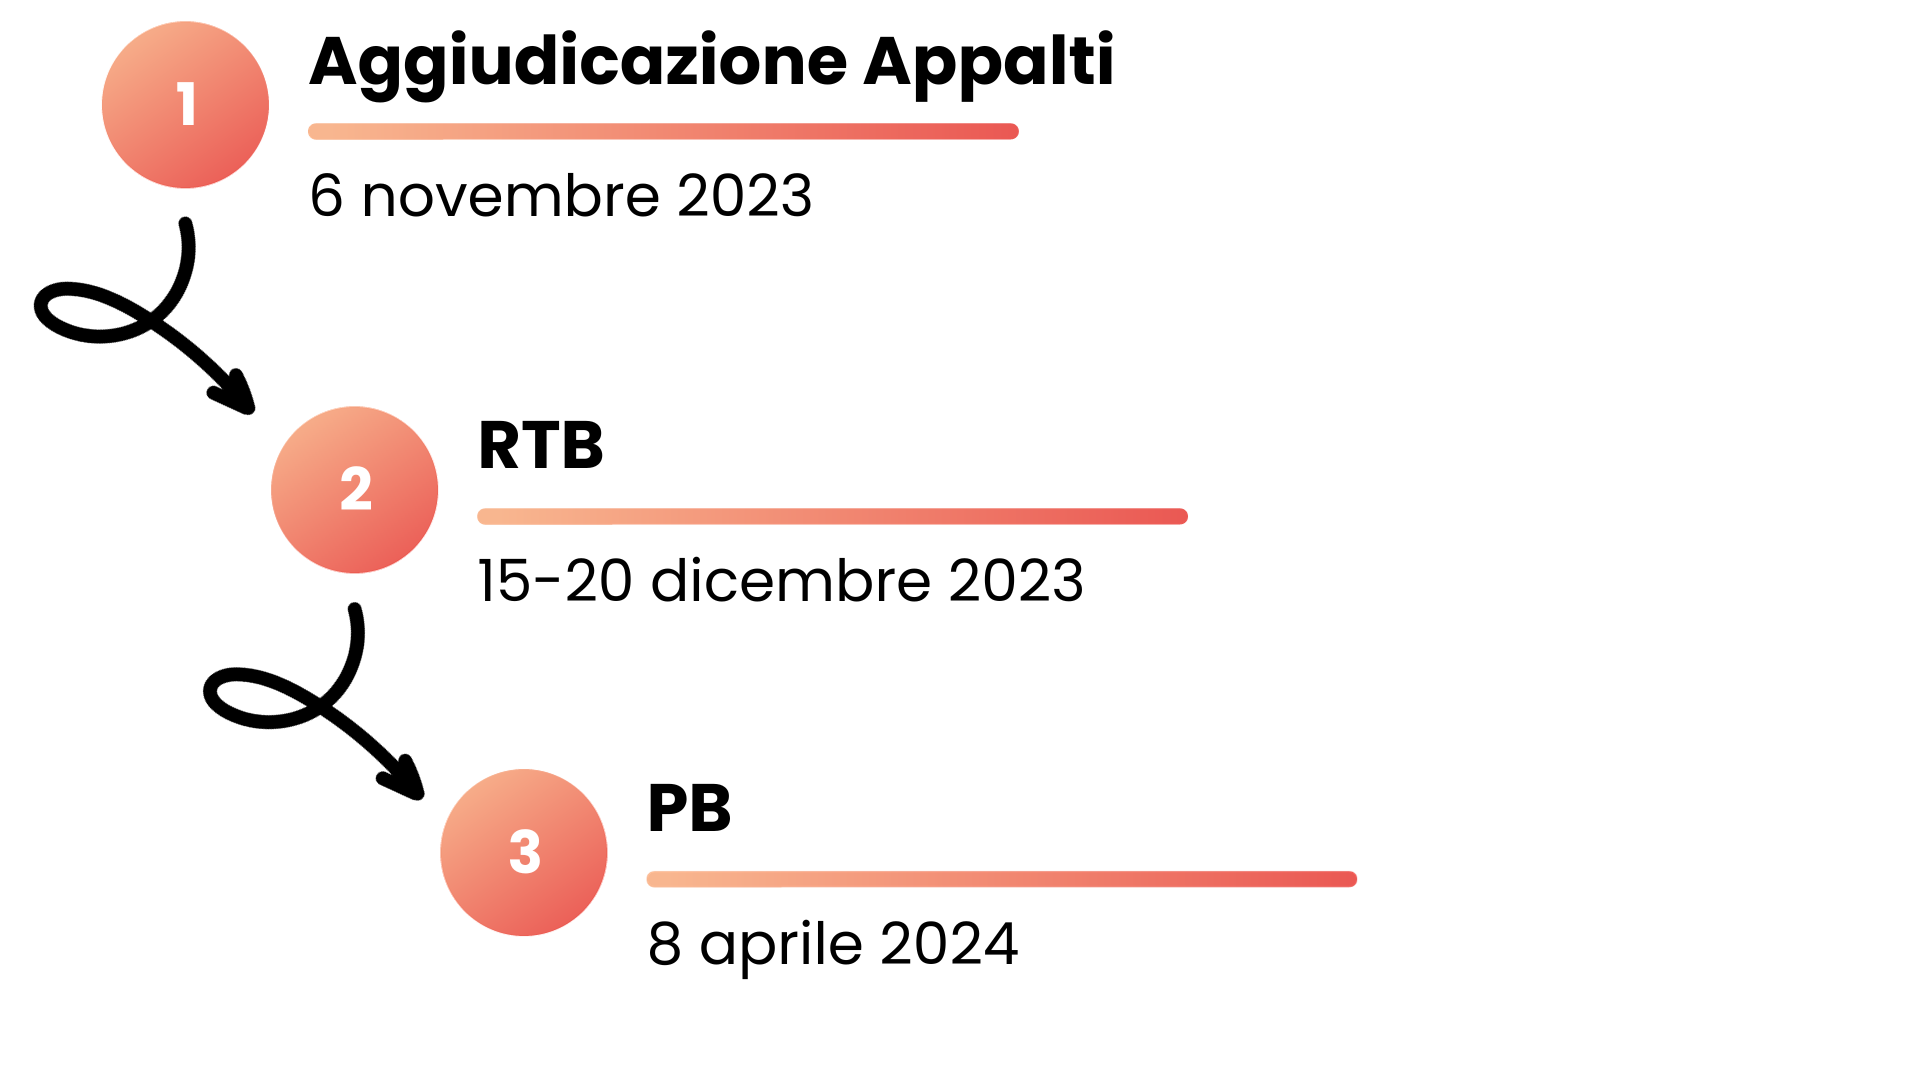
\includegraphics[width=10cm]{Calendario di massima - prima stesura.png}
        \caption{Grafico calendario - prima stesura}
    \end{figure}
\begin{comment}    
{\renewcommand{\arraystretch}{1.5}
\begin{table}[H]
\begin{tabularx}{\textwidth}{X|X}
\textbf{Revisione} & \textbf{Data} \\
\hline
Requirements \& Technology Baseline & \color{red} Periodo da $2023-12-15$ a $2023-12-20$ \color{black}\\
\hline
Product Baseline &  $2024-04-08$\\

\end{tabularx}
\caption{Tabella calendario di massima - prima stesura}
\end{table}}
\end{comment}




\section{Stima dei costi di realizzazione}
\paragraph{}In questa sezione vengono riportate le stime dei costi e degli impegni orari alla luce di quanto analizzato nelle sezioni di \hyperref[section:Rischi]{\textbf{Rischi e mitigazione}} e \hyperref[section:Pianificazione]{\textbf{Pianificazione}}.

\subsection{Prima stesura 2023-11-23}
\paragraph{}La stima dei costi di realizzazione non viene intaccata in maniera significativa dal cambiamento del calendario.

{\renewcommand{\arraystretch}{1.2}
\begin{table}[H]
\begin{tabularx}{\textwidth}{c|X|X|X|X|X|X|X}
        \textbf{Membri} & $\operatorname{\textbf{Re}}$ & $\mathrm{\textbf{Am}}$ & \textbf{An} & \textbf{Proj} & \textbf{Prgm} & \textbf{Ver} & \textbf{Tot} \\
        \hline Bresolin G. & 9 & 9 & 8 & 13 & 31 & 24 & 94 \\
        \hline Ciriolo I. & 11 & 11 & 10 & 16 & 27 & 19 & 94 \\
        \hline Campese M. & 10 & 10 & 8 & 15 & 26 & 25 & 94 \\
        \hline Dugo A. & 11 & 8 & 8 & 15 & 28 & 24 & 94 \\
        \hline Feltrin E. & 11 & 9 & 10 & 12 & 28 & 24 & 94 \\
        \hline Michelon R. & 9 & 8 & 10 & 13 & 30 & 24 & 94 \\
        \hline Orlandi G. & 9 & 8 & 9 & 14 & 26 & 28 & 94 
    \end{tabularx}
    \caption{Tabella distribuzione ore - prima stesura}
    \end{table}
\paragraph{Schema a torta di distribuzione ore ruoli} Di seguito viene illustrata in maniera immediata la redistribuzione delle ore nei ruoli di progetto.
    \begin{figure}[!h]
        \centering
        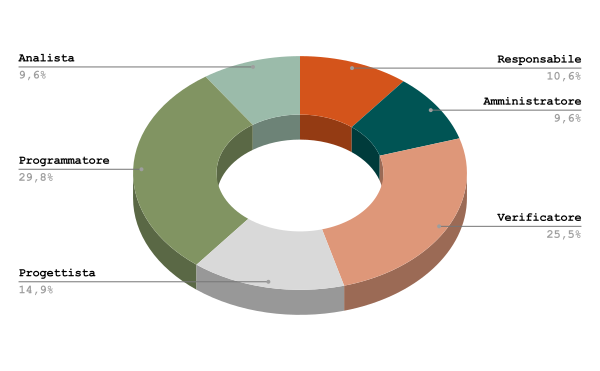
\includegraphics[width=10cm]{torta.png}
        %\includesvg{torta 1}
        \caption{Grafico ore percentuali - prima stesura}
        
    \end{figure}


\section{Rischi e loro mitigazione}
\label{section:Rischi}
\paragraph{}Questa sezione di occupa di analizzare le difficoltà che si possono verificare durante lo svolgimento del progetto e che possono avere influenze sulla pianificazione delle attività, portando a rallentamenti e ostacoli nell'avanzamento.\\
Per poter individuare e gestire questi rischi, vengono di seguito esaminati e corredati da descrizione, previsione della loro occorrenza, grado di pericolosità e infine da misure di mitigazione degli effetti negativi nel caso si verifichino.
I rischi sono indicati con la notazione seguente: \\ R[Tipo]-[Numero] \ \  
\begin{itemize}
\item \textbf{R} sta per \textit{Rischio};
\item \textbf{Tipo} indica il tipo che può essere tra i seguenti:
    \begin{itemize}
	\item \textbf{P} (Personale);
	\item \textbf{O} (Organizzativo);
	\item \textbf{T} (Tecnologico).
    \end{itemize}
\item \textbf{Numero} indica il numero in quella categoria.
\end{itemize}


%PERSONALI

\subsection{Rischi personali}

% RISCHIO IMPEGNI PERSONALI

\subsubsection{Impegni e problemi personali}
{\renewcommand{\arraystretch}{1.5}
\begin{table}[H]
\begin{tabularx}{\textwidth}{c|X}
\textbf{ID Rischio} & RP-1 \\
\hline
\textbf{Rischio} & Impegni e problemi personali\\
\hline
\textbf{Descrizione} & Ogni componente del team ha impegni esterni e può avere problemi strettamente personali. Questo indica che qualche membro può non essere disponibile in certi momenti.\\
\hline
\textbf{Occorrenza} & Media\\
\hline
\textbf{Impatto} & Alto\\
\hline
\textbf{Misure di mitigazione} & I membri interessati si impegnano ad avvisare tempestivamente il gruppo; per far fronte a tale rischio si coprirà l’intervallo non produttivo del componente con una suddivisione omogenea tra i restanti colleghi delle attività rimaste in sospeso.
Riuscire a non spostare la \textit{milestone} è prioritario.\\
\end{tabularx}
\caption{Tabella rischi imprevisti e impegni personali}
\end{table}}




\subsubsection{Problemi fra i membri del gruppo}

{\renewcommand{\arraystretch}{1.5}
\begin{table}[H]
\begin{tabularx}{\textwidth}{c|X}
\textbf{ID Rischio} & RP-2 \\
\hline
\textbf{Rischio} & Problemi fra i membri del gruppo  \\
\hline
\textbf{Descrizione} & Possono verificarsi divergenze di pensiero tra i componenti del gruppo che rischiano di portare a discussioni. \\
\hline
\textbf{Occorrenza} & Media\\
\hline
\textbf{Impatto} & Medio \\
\hline
\textbf{Misure di mitigazione} & Le parti prese in causa esporranno il loro punto di vista in maniera educata; il Responsabile è tenuto a fare da moderatore. \\
\end{tabularx}
\caption{Tabella divergenze interne}
\end{table}
}


%ORGANIZZATIVI

\subsection{Rischi organizzativi}

\subsubsection{Sottostima del tempo necessario per una attività}

{\renewcommand{\arraystretch}{1.5}
\begin{table}[h]
\begin{tabularx}{\textwidth}{c|X}
\textbf{ID Rischio} & RO-1 \\
\hline
\textbf{Rischio} & Sottostima del tempo necessario per una attività\\
\hline
\textbf{Descrizione} & Il team può andare in contro ad una sottostima del tempo necessario per il soddisfacimento di un requisito o di un' attività.\\
\hline
\textbf{Occorrenza} & Alta\\
\hline
\textbf{Impatto} & Alto\\
\hline
\textbf{Misure di mitigazione} & Tale errore deve essere reso noto al team tempestivamente; chi ha disponibilità viene incaricato di fornire assistenza per minimizzare il ritardo nel completamento dell'obiettivo.\\
\end{tabularx}
\caption{Tabella sottostima del tempo}
\end{table}

\subsubsection{Stima errata dei costi}

{\renewcommand{\arraystretch}{1.5}
\begin{table}[H]
\begin{tabularx}{\textwidth}{c|X}
\textbf{ID Rischio} & RO-2 \\
\hline
\textbf{Rischio} & Stima errata dei costi \\
\hline
\textbf{Descrizione} & Potrebbe verificarsi una valutazione scorretta dei costi di incarico.\\
\hline
\textbf{Occorrenza} & Media\\
\hline
\textbf{Impatto} & Medio\\
\hline
\textbf{Misure di mitigazione} & Si provvederà a far uso dei diagrammi di Gantt per l'organizzazione delle attività lasciando dello "slack" tra le attività con dipendenze.\\
\end{tabularx}
\caption{Tabella stima errata dei costi}
\end{table}



\subsubsection{Disponibilità di lavoro non sfruttato}

{\renewcommand{\arraystretch}{1.5}
\begin{table}[H]
\begin{tabularx}{\textwidth}{c|X}
\textbf{ID Rischio} & RO-3 \\
\hline
\textbf{Rischio} & Disponibilità di lavoro non sfruttato \\
\hline
\textbf{Descrizione} & Caso in cui un membro del team si ritrova del tempo produttivo "libero" senza attività assegnate al proprio ruolo che lo impegnino.\\
\hline
\textbf{Occorrenza} & Media\\
\hline
\textbf{Impatto} & Medio\\
\hline
\textbf{Misure di mitigazione} & Il membro del team in questione viene invitato a farsi avanti e ad aiutare i membri in difficoltà o a farsi carico di attività non ancora assegnate anche non necessariamente legate al proprio ruolo in quel determinato \textit{sprint}. \\

\end{tabularx}
\caption{Tabella disponibilità non sfruttata}
\end{table}



%TECNOLOGICI

\subsection{Rischi tecnologici}

\subsubsection{Scarsa esperienza con le tecnologie del progetto}

{\renewcommand{\arraystretch}{1.5}
\begin{table}[H]
\begin{tabularx}{\textwidth}{c|X}
\textbf{ID Rischio} & RT-1 \\
\hline
\textbf{Rischio} & Scarsa esperienza con le tecnologie del progetto \\
\hline
\textbf{Descrizione} & Si possono verificare difficoltà di utilizzo di strumenti di lavoro o inesperienze\\
\hline
\textbf{Occorrenza} & Alta\\
\hline
\textbf{Impatto} & Alta\\
\hline
\textbf{Misure di mitigazione} & Il rischio non può essere evitato, dato che una buona esperienza con le tecnologie si ottiene con gli anni (tempo non a disposizione per questo progetto comunque complesso). Il primo passo è la comunicazione interna delle difficoltà più gravi.
\begin{itemize}
    \item Se le lacune riguardano le tecnologie usate abitualmente da AzzurroDigitale, è possibile richiedere un colloquio di formazione o supporto;
    \item Se le tecnologie sono note solo ad alcuni membri del gruppo, questi si impegnano a realizzare dei workshop per portare a regime le conoscenze degli altri componenti;
    \item Nel caso si parli di una tecnologia sconosciuta a tutti i membri, si prosegue cercando e studiando la guida utente e la documentazione associata.
\end{itemize}
\end{tabularx}
\caption{Tabella scarsa esperienza tecnologica}
\end{table}


\subsubsection{Guasti hardware e problematiche software}

{\renewcommand{\arraystretch}{1.5}
\begin{table}[H]
\begin{tabularx}{\textwidth}{c|X}
\textbf{ID Rischio} & RT-2 \\
\hline
\textbf{Rischio} & Guasti hardware e problematiche software \\
\hline
\textbf{Descrizione} & Si potrebbero presentare difficoltà legate all’hardware o al software utilizzati per cui un membro del gruppo risulta ostacolato nel portare a compimento un obiettivo o una attività. \\
\hline
\textbf{Occorrenza} & Bassa \\
\hline
\textbf{Impatto} & Medio\\
\hline
\textbf{Misure di mitigazione} & Comunicare tempestivamente il guasto al gruppo e se necessario chiedere aiuto e condivisione di un mezzo funzionante.\\
\end{tabularx}
\caption{Tabella guasti hardware e software}
\end{table}


\subsection{Valutazione efficacia delle misure}
\paragraph{}Questa sezione riassume la sezione di analisi dei rischi e valuta l'efficacia delle pratiche di mitigazioni degli stessi nel caso questi si siano verificati.\\
{\renewcommand{\arraystretch}{1.5}
\begin{table}[H]
\begin{tabularx}{\textwidth}{c|c|c|X}
\textbf{ID Rischio} & \textbf{Occorrenza effettiva} & \textbf{Impatto effettivo} & \textbf{\quantities{Efficacia misure di \\mitigazione}} \\
\hline
RP-1 & - & - & -\\
\hline
RP-2 & - & - & - \\
\hline
RO-1 & - & - & -\\
\hline
RO-2 & - & - & -\\
\hline
RO-3 & - & - & -\\
\hline
RT-1 & - & - & -\\
\hline
RT-2 & - & - & -\\


\end{tabularx}
\caption{Tabella riassuntiva delle misure di mitigazione}
\end{table}


\section{Pianificazione e modello di sviluppo}
\label{section:Pianificazione}

\paragraph{}Il team decide di adottare il modello di sviluppo \textit{Agile} 
promuovendo un approccio incrementale al lavoro; questo consentirà di suddividere il progetto in compiti più gestibili, ovvero \textit{sprint}, ciascuno dei quali produrrà risultati funzionanti. Questo consente al team di progetto di reagire ai cambiamenti in modo più efficace.\\
\paragraph{}I periodi individuati sono \textit{sprint} di 14 giorni con seguente rotazione dei ruoli assunti dai componenti del gruppo.\\
Questo tipo di pianificazione permette di avere un orizzonte temporale limitato; ciò aiuta nel caso in cui vengano riscontrate difficoltà che causano danni ad attività che dipendono le une dalle altre, è possibile contenere questi ultimi e riorganizzare le attività nel periodo successivo.
\subsection{Requirements and Technology Baseline}
\paragraph{}Questo periodo antecedente la revisione RTB di progetto si focalizza sulla preparazione dei documenti (Analisi dei requisiti, Piano di progetto, Piano di qualifica, ampliamento Norme di progetto) e alla creazione del Proof of Concept per il progetto.

\subsubsection{Periodo da 2023-11-07 a 2023-11-21}
\paragraph{}Questo primo periodo segue l'assegnazione dei capitolati e viene utilizzato principalmente per configurare l'ambiente di lavoro, le norme e per studiare i casi d'uso e perseguire l'analisi dei requisiti del progetto. Infine lo \textit{sprint} si concentra sullo studio e selezione di tecnologie utili allo sviluppo del progetto.
\paragraph{Obiettivi}
\begin{itemize}
    \item Stesura e ampliamento delle Norme di progetto;
    \item Prima stesura Analisi dei requisiti;
    \item Automazione versionamento;
    \item Manutenzione ambiente di lavoro;
    \item Software selection;
    \item Verbali delle riunioni.
        
\end{itemize}
%\paragraph{Diagramma di Gantt}
\vspace{1em}

 \begin{figure}[H]
        \centering        
        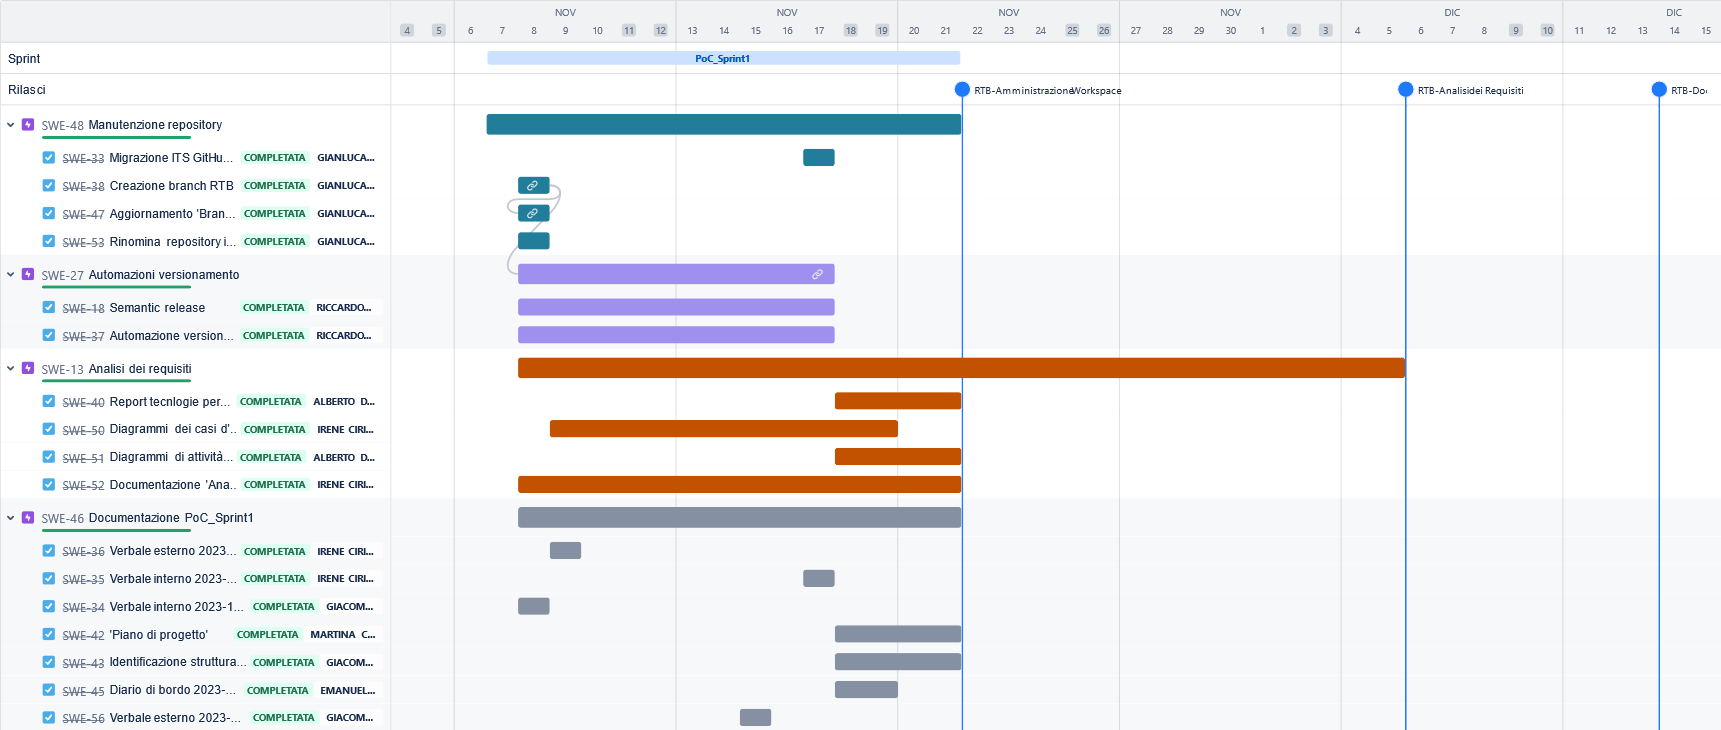
\includegraphics[width=15.5cm]{periodo1.png}
        \caption{Diagramma di Gantt da 2023-11-07 a 2023-11-21 }
    \end{figure}
%\paragraph{Ruoli:} (vanno messi nel consuntivo chi e per quante ore?)


\subsubsection{Periodo da 2023-11-21 a 2023-12-05}
\paragraph{}In questo periodo le ore di lavoro sono concentrate nella creazione di un PoC richiesto dall'azienda e nell'ampliamento e miglioramento della documentazione necessaria per guidare l'avanzamento del progetto.
\paragraph{Obiettivi}
\begin{itemize}
    \item Progettazione PoC;
    \item Codifica PoC ;
    \item Prosecuzione stesura Analisi dei requisiti;
    \item Migliorie Norme di progetto e Piano di progetto;
    \item Stesura correttiva Piano di qualifica.
  
\end{itemize}
%\paragraph{Diagramma di Gantt}

\subsubsection{Periodo da 2023-12-05 a 2023-12-19}





\subsection{Product Baseline}



\subsubsection{Periodo da 2023-12-19 a 2024-01-02}



\subsubsection{Periodo da 2024-01-02 a 2024-01-16}



\subsubsection{Periodo da 2024-01-16 a 2024-01-30}



\subsubsection{Periodo da 2024-01-30 a 2024-02-13}



\subsubsection{Periodo da 2024-02-13 a 2024-02-27}



\subsubsection{Periodo da 2024-02-27 a 2024-03-12}


\subsubsection{Periodo da 2024-03-12 a 2024-03-26}



\subsubsection{Periodo da 2024-03-26 a 2024-04-09}



\section{Preventivo}

%Per queste voci si rimanda al documento “Preventivo costi e assunzione impegni”, presente nella repository Presentazio




\section{Consuntivo}


\subsubsection{Periodo da 2023-11-07 a 2023-11-21}


\begin{table}[H]
\begin{tabularx}{\textwidth}{c|X|X|X|X|X|X|X}
        \textbf{Membri} & $\operatorname{\textbf{Re}}$ & $\mathrm{\textbf{Am}}$ & \textbf{An} & \textbf{Proj} & \textbf{Prgm} & \textbf{Ver} & \textbf{Tot} \\
        \hline Bresolin G. & 0& 4 & 1 & 0 & 0 & 0 & 5 \\
        \hline Ciriolo I. & 0 & 0 & 5 & 0 & 0 & 1 & 6 \\
        \hline Campese M. & 0 & 1 & 0 & 0 & 0 & 8 & 9 \\
        \hline Dugo A. & 0 & 3 & 0 & 0 & 0 & 0 & 3 \\
        \hline Feltrin E. & 4 & 0 & 0 & 0 & 0 & 0 & 4 \\
        \hline Michelon R. & 0 & 4 & 0 & 0 & 0 & 0 & 4 \\
        \hline Orlandi G. & 0 & 0 & 3 & 0 & 0 & 1 & 4 \\
        \hline
        \textbf{Totale ruolo} & 4 & 12 & 9 & 0 & 0 & 10 & - 
    \end{tabularx}
    \caption{Consuntivo ore - da 2023-11-07 a 2023-11-21}
    \end{table}
    






\subsubsection{Periodo da 2023-11-21 a 2023-12-05}

\subsubsection{Periodo da 2023-12-05 a 2023-12-19}


\subsubsection{Periodo da 2023-12-19 a 2024-01-02}



\subsubsection{Periodo da 2024-01-02 a 2024-01-16}



\subsubsection{Periodo da 2024-01-16 a 2024-01-30}



\subsubsection{Periodo da 2024-01-30 a 2024-02-13}



\subsubsection{Periodo da 2024-02-13 a 2024-02-27}



\subsubsection{Periodo da 2024-02-27 a 2024-03-12}


\subsubsection{Periodo da 2024-03-12 a 2024-03-26}



\subsubsection{Periodo da 2024-03-26 a 2024-04-09}


\section{Retrospettiva generale}
\subsection{Gestione delle risorse}
\subsubsection{Tempo}
\subsubsection{Budget}
\subsection{Aspetti positivi}
\subsection{Aspetti negativi}
%\color{gray}\paragraph{}pratica del vincolo di un ruolo, può non far sfruttare tutta la disponibilità di lavoro dei componenti, etc.
%\color{black}
\subsection{Conclusioni}

\end{document}